\documentclass[11pt]{article}

\usepackage[a4paper,margin=2.6cm]{geometry}
\usepackage[T1]{fontenc}
\usepackage[utf8]{inputenc}
\usepackage{lmodern}
\usepackage{microtype}
\usepackage{amsmath,amssymb}
\usepackage{booktabs}
\usepackage{graphicx}
\usepackage{xcolor}
\usepackage[font=small,labelfont=bf]{caption}
\usepackage{enumitem}
\definecolor{linkblue}{HTML}{1c5cab}
\usepackage[colorlinks=true,linkcolor=linkblue,citecolor=linkblue,urlcolor=linkblue]{hyperref}

\newcommand{\sillage}{\textsc{Sillage}}
\newcommand{\dnll}{\Delta\mathrm{NLL}}
\newcommand{\ci}[2]{{\footnotesize[#1,\,#2]}}

\title{\bfseries Memory Remembers, Fast Weights Adapt:\\
Two Gradient-Free Ways to Learn at Test Time,\\
and Why They Add Up}
\author{Abderrahmane Sghairi\\
\small Independent Researcher, Issoire, France\\
\small \texttt{sghairipro63@gmail.com}}
\date{August 2026}

\begin{document}
\maketitle

\begin{abstract}
A frozen language model can be improved at inference in two very different gradient-free ways: by \emph{remembering} what it just read in an associative store, or by \emph{adapting} its readout with fast weights. We implement the second as a rank-$r$ delta-rule adapter on the output layer --- $\ell' = \ell + A\varphi(h)$ with $A \leftarrow A + \eta\,(\mathbf{1}_{x} - p')\varphi(h)^{\!\top}$, a local update that transports no error through any layer --- and compare it head-to-head, and in combination, with a fixed-size Hebbian memory, under a strictly prequential protocol on two frozen models (GPT-2 124M, Qwen3-0.6B) and four streams (36k--500k tokens). Three findings. \textbf{(1) A regime inversion.} On novel, highly repetitive text the memory dominates ($+0.472$ vs $+0.237$ nats on GPT-2; $+0.244$ vs $+0.082$ on Qwen3); on low-repetition text the ordering flips by up to $20\times$ in the adapter's favour ($+0.077$ vs $+0.004$ nats on Qwen3/Einstein). Memory captures verbatim recurrence; fast weights retune the readout to the document's style and vocabulary. \textbf{(2) They add up.} Routing the memory on top of the adapted base recovers 89--96\% of the sum of the two standalone gains on every stream (paired block-bootstrap $P = 1.000$ in all six configurations); on the manuscripts stream the combination reaches $+0.633$ nats, perplexity $31.2 \to 16.6$. \textbf{(3) Rank 16 suffices}, making the adapter 3.2\,MB on GPT-2 (9.7\,MB on Qwen3) --- comparable to the 4.2\,MB memory --- for 93--96\% of the rank-256 gain. We also report a clean negative result that maps the boundary of a signal used throughout this line of work: \emph{surprise gating, which is what makes the Hebbian memory work, hurts the delta rule} (Manuscripts $+0.195$ vs $+0.237$ uniform; Einstein $-0.000$ vs $+0.075$), because the delta rule already carries its own error term and gating double-counts it. A 500k-token run shows no drift and no divergence: per-50k gains rise from $+0.040$ to $+0.072$ nats and stay there. Code and all controls are released.
\end{abstract}

\section{Introduction}

Two companion systems gave frozen language models gradient-free test-time learning through \emph{memory}: a fixed-size Hebbian matrix with surprise-gated amplitude writes \cite{sillage}, extended with semantic keys and score-level routing \cite{router} and with a consolidating cold tier \cite{hier}. All of them \emph{store and retrieve}; none of them \emph{change the model}.

The complementary idea is old: \emph{fast weights} \cite{hinton1987,schmidhuber1992,ba2016} adapt a network's own parameters on the timescale of the input. Modern test-time-training systems \cite{ttt,titans,ttr} pursue this with gradient-based inner loops. This paper asks the narrower question that fits the gradient-free program: can a purely \emph{local} update of the output layer --- the delta rule, with no error transported through any layer --- improve a frozen LM at inference, and does it \emph{add} to what memory already provides, or merely duplicate it?

The answer is a clean division of labour, which we quantify. Fast weights and memory dominate opposite regimes, and their gains are nearly additive when combined --- so the right architecture is not one or the other but both, at a total cost of a few megabytes.

\paragraph{Contributions.}
\begin{enumerate}[leftmargin=1.5em,itemsep=2pt]
\item \textbf{A gradient-free readout adapter} for frozen LMs (\S\ref{sec:method}): a rank-$r$ delta-rule update on the output layer, prequentially evaluated, improving two frozen models on four streams (\S\ref{sec:regimes}).
\item \textbf{The regime inversion} (\S\ref{sec:regimes}): memory wins on novel repetitive text, fast weights win by up to $20\times$ on low-repetition text --- replicated across both models.
\item \textbf{Additivity} (\S\ref{sec:additivity}): the combination recovers 89--96\% of the sum of the parts, $P = 1.000$ in all six model$\times$stream configurations; new best result on the manuscripts stream ($+0.633$ nats, PPL $31.2 \to 16.6$).
\item \textbf{Rank-16 sufficiency} (\S\ref{sec:rank}): 3.2\,MB (GPT-2) / 9.7\,MB (Qwen3) buys 93--96\% of the rank-256 gain, putting the adapter in the same budget class as the memory.
\item \textbf{A boundary for the surprise signal} (\S\ref{sec:gating}): the gate that makes Hebbian writing, routing and consolidation work \cite{sillage,router,hier} \emph{hurts} the delta rule, for an identifiable reason. Three validated roles, one refuted --- reported rather than buried.
\item \textbf{Long-horizon stability} (\S\ref{sec:stability}): 500k tokens with no drift or divergence, in a rule whose learning rate is otherwise fragile ($\eta \ge 0.3$ diverges).
\end{enumerate}

\section{Method}\label{sec:method}

\subsection{The adapter}

Let $h_j \in \mathbb{R}^{d}$ be the frozen model's final hidden state at position $j$ and $\ell_j \in \mathbb{R}^{|\mathcal{V}|}$ its logits. Fix a random projection $R \in \mathbb{R}^{d \times r}$ and let $\varphi_j = R^{\!\top}h_j / \Vert R^{\!\top}h_j\Vert$. The adapter is a matrix $A \in \mathbb{R}^{|\mathcal{V}| \times r}$, initialized at zero, that shifts the logits and is updated by the delta rule:
\begin{align}
\ell'_j &= \ell_j + A\,\varphi_j, \qquad p'_j = \mathrm{softmax}(\ell'_j),\\
A &\leftarrow A + \eta\,\big(\mathbf{1}_{x_{j+1}} - p'_j\big)\,\varphi_j^{\!\top}.
\label{eq:delta}
\end{align}
Equation~\eqref{eq:delta} is the exact cross-entropy gradient \emph{at the readout}, and nothing else: no error is transported into the transformer, no activation is stored for a backward pass, and the frozen weights never move. The update is one rank-1 outer product per token, and the state is $|\mathcal{V}|\,r$ floats.

\textbf{Protocol.} Strictly prequential: at every position the token is scored with the \emph{current} $A$, and only then is $A$ updated. Hyperparameters ($\eta$, gating, rank) are selected on the first 20\% of each stream and frozen; all numbers are reported on the remaining 80\%, with 95\% block-bootstrap confidence intervals (512-token blocks) and paired tests on identical positions, exactly as in \cite{sillage,router,hier}.

\subsection{The memory, and how the two are combined}

The memory is the $n$-gram tier of \cite{sillage}: a $4096\times256$ Hebbian matrix ($4.2$\,MB), addressed by sliding 4-gram bindings of random token hypervectors, written with surprise-gated amplitude updates. Combination reuses the score-level router of \cite{router}: the memory's distribution is mixed into the \emph{adapted} base where its confidence clears a dev-tuned threshold,
\[
p = \mathbf{1}[\text{mem confident}]\;\lambda\,p_{\mathrm{mem}} + \big(1 - \mathbf{1}[\cdot]\lambda\big)\,p',
\]
with $(\beta, \lambda, \text{threshold})$ re-tuned on dev for each base. Nothing else changes, so any difference is attributable to the adapter.

\section{Experiments}

Frozen GPT-2 124M and Qwen3-0.6B; streams from \cite{sillage}: \textsc{Manuscripts} (36k tokens of unpublished technical drafts, novel to both models, 35\% of positions repeating an earlier 4-gram), \textsc{Einstein} and \textsc{Alice} (40k-token classics), \textsc{War and Peace} (500k tokens). Base perplexities: $31.2$, $17.6$, $13.9$, $24.4$ (GPT-2); $14.9$, $13.0$ (Qwen3).

\subsection{The regime inversion}\label{sec:regimes}

\begin{figure}[t]
\centering
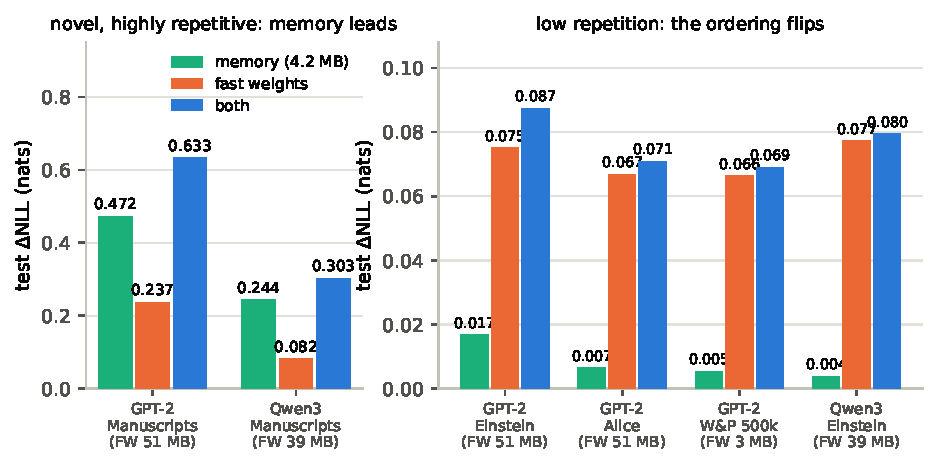
\includegraphics[width=\linewidth]{figs/p4fig1_regimes.pdf}
\caption{Memory, fast weights, and their combination. Left: on novel, highly repetitive text the memory leads on both models. Right: on low-repetition streams the ordering flips --- by $4.5\times$ (GPT-2/Einstein), $10\times$ (GPT-2/Alice), $12\times$ (GPT-2/W\&P) and $20\times$ (Qwen3/Einstein) in the adapter's favour. Note the different vertical scales.}
\label{fig:regimes}
\end{figure}

\begin{table}[t]
\centering\small
\caption{Test $\dnll$ (nats) over the frozen model. FW = the delta-rule adapter (uniform step, best rank on dev); memory = the 4.2\,MB Hebbian tier; ``both'' = memory routed on the adapted base. Paired column: ``both'' vs memory alone, block bootstrap; every entry has $P = 1.000$. Additivity = ``both'' as a fraction of (FW $+$ memory).}
\label{tab:main}
\begin{tabular}{@{}llccccc@{}}
\toprule
model & stream & memory & FW & both & paired $\Delta$ vs memory & additivity\\
\midrule
GPT-2 & \textsc{Manuscripts} & $\mathbf{+0.472}$ & $+0.237$ & $+0.633$ & $+0.161$ \ci{0.142}{0.183} & 89\%\\
GPT-2 & \textsc{Einstein} & $+0.017$ & $\mathbf{+0.075}$ & $+0.088$ & $+0.071$ \ci{0.061}{0.080} & 95\%\\
GPT-2 & \textsc{Alice} & $+0.007$ & $\mathbf{+0.067}$ & $+0.071$ & $+0.064$ \ci{0.059}{0.070} & 96\%\\
GPT-2 & \textsc{W\&P} 500k & $+0.006$ & $\mathbf{+0.066}$ & $+0.069$ & $+0.064$ \ci{0.061}{0.066} & 96\%\\
Qwen3 & \textsc{Manuscripts} & $\mathbf{+0.244}$ & $+0.082$ & $+0.303$ & $+0.059$ \ci{0.051}{0.069} & 93\%\\
Qwen3 & \textsc{Einstein} & $+0.004$ & $\mathbf{+0.077}$ & $+0.080$ & $+0.076$ \ci{0.069}{0.082} & 98\%\\
\bottomrule
\end{tabular}
\end{table}

Figure~\ref{fig:regimes} and Table~\ref{tab:main} give the central result. The two mechanisms are not competitors on a single axis: which one wins is decided by the stream, and the gap is large in both directions. On \textsc{Manuscripts} --- text neither model has seen, in which one position in three repeats an earlier 4-gram --- the memory is $2$--$3\times$ the adapter. On the classics and on long narrative, where verbatim recurrence is scarce, the adapter is $4.5$ to $20\times$ the memory; on Qwen3/\textsc{Einstein} the memory is essentially inert ($+0.004$) while the adapter delivers $+0.077$.

The interpretation is straightforward. The Hebbian tier can only fire when an exact 4-gram returns, so its value tracks verbatim repetition. The adapter has no notion of repetition at all: it performs an online logistic regression from a random 16--256 dimensional summary of the model's own hidden state to the next token, which is exactly a recalibration of the readout to the document's register, terminology and orthographic conventions. Notably, the adapter's gain is remarkably \emph{stable across streams} on a given model (GPT-2: $0.066$--$0.075$ on the three non-manuscript streams; Qwen3: $0.077$--$0.082$ on both), whereas the memory's swings by two orders of magnitude ($0.004$ to $0.472$). Adaptation is a broad, shallow win; memorization is a narrow, deep one.

\subsection{The gains add up}\label{sec:additivity}

Combining is nearly free of interference: ``both'' recovers 89--96\% of the arithmetic sum of the standalone gains (Table~\ref{tab:main}, last column), and improves on memory alone with $P = 1.000$ in all six configurations. On \textsc{Manuscripts} with GPT-2 the combination reaches $+0.633$ nats --- perplexity $31.2 \to 16.6$ --- which is, to our knowledge, the strongest gradient-free improvement reported on that stream, exceeding the memory-only state of the art of \cite{sillage,router} by 34\%. The router that arbitrates them is unchanged from \cite{router}; only the base distribution it sits on has been adapted.

That near-additivity is itself evidence about what the two mechanisms encode: had the adapter been implicitly memorizing recurrences, the memory would have found little left to contribute on \textsc{Manuscripts}, yet it still adds $+0.161$ nats there on top of a fully adapted base.

\subsection{Rank 16 is enough}\label{sec:rank}

\begin{figure}[t]
\centering
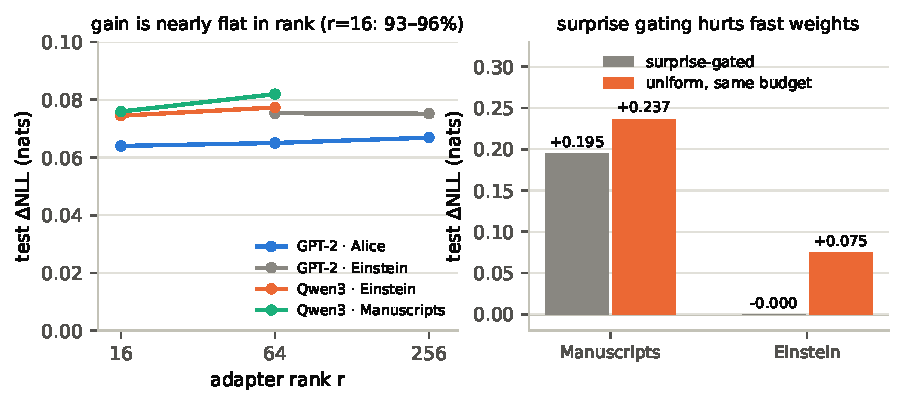
\includegraphics[width=\linewidth]{figs/p4fig3_ablations.pdf}
\caption{Left: the adapter's gain is nearly flat in rank --- $r = 16$ keeps 93--96\% of the $r = 256$ gain on every model$\times$stream pair tested. Right: surprise gating, the signal that makes Hebbian memory work, \emph{costs} the delta rule 18\% of its gain on \textsc{Manuscripts} and all of it on \textsc{Einstein}.}
\label{fig:ablations}
\end{figure}

Adapter size is $|\mathcal{V}|\,r$ floats, so rank decides whether this mechanism is deployable next to a 4.2\,MB memory. Figure~\ref{fig:ablations} (left) shows the gain is almost flat in $r$: on GPT-2/\textsc{Alice}, $r = 16/64/256$ give $+0.0640/+0.0650/+0.0669$; on GPT-2/\textsc{Einstein}, $r = 64$ matches $r = 256$ exactly ($+0.0753$ vs $+0.0752$); on Qwen3, $r = 16$ keeps 93--96\% of $r = 64$. At $r = 16$ the adapter is \textbf{3.2\,MB} on GPT-2 and 9.7\,MB on Qwen3 (whose vocabulary is $3\times$ larger) --- the same budget class as the memory it complements, and $16\times$ smaller than the $r = 256$ adapter with which we began. The useful test-time signal in the readout is low-rank.

\subsection{Surprise gating helps memory and hurts fast weights}\label{sec:gating}

Across this line of work a single free scalar --- the model's own token surprise $g = -\ln p_{\mathrm{LM}}$ --- has done three jobs: scaling Hebbian writes \cite{sillage}, earning routing confidence \cite{router}, and ranking consolidation into a cold store \cite{hier}. It is natural to try it as the adapter's learning-rate gate, $\eta \to \eta\,g$. It fails, and the failure replicates (Figure~\ref{fig:ablations}, right): on \textsc{Manuscripts} the gated rule scores $+0.195$ against $+0.237$ for a uniform step of matched total plasticity budget ($\eta\,\bar{g}$), and on \textsc{Einstein} gating removes the entire effect ($-0.000$ vs $+0.075$). The uniform variant also wins on dev, so the protocol selects it without hindsight.

The reason is structural. The delta rule's update is already proportional to its own error, $(\mathbf{1}_{x} - p')$, which is large exactly when the token was unexpected. Multiplying by $g = -\ln p$ therefore double-counts surprise, over-weighting rare and noisy events --- the same over-weighting bias measured for Hebbian writes in \cite{sillage}, but here with no compensating benefit, since the rule needs no external signal to know when it was wrong. Hebbian storage, which writes with equal strength regardless of correctness, does need one. \emph{Gate the mechanisms that cannot see their own error; leave alone the ones that can.}

\subsection{Long-horizon stability}\label{sec:stability}

\begin{figure}[t]
\centering
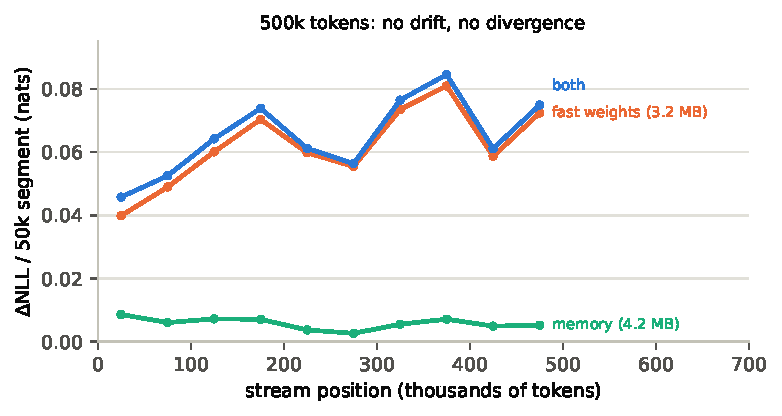
\includegraphics[width=0.8\linewidth]{figs/p4fig2_stability.pdf}
\caption{500k tokens of \emph{War and Peace} (GPT-2, $r = 16$, 3.2\,MB): per-50k-token gains for the adapter, the memory, and their combination. The adapter's gain grows early and then plateaus around $+0.07$ nats; there is no drift, no decay and no divergence.}
\label{fig:stability}
\end{figure}

Online learning rules with a fixed step are fragile: at $\eta = 0.3$ the adapter loses half its gain and at $\eta = 1.0$ it diverges catastrophically ($-0.525$ nats). The question is therefore whether the selected $\eta = 0.1$ survives a long stream. Figure~\ref{fig:stability} answers it: over 500k tokens the per-50k gain climbs from $+0.040$ to a plateau of $+0.055$--$+0.081$ and ends at $+0.072$, with the aggregate $+0.066$ \ci{0.064}{0.069}. The adapter neither saturates like a fixed-size memory \cite{sillage} nor runs away; combined with the memory it holds $+0.069$ over the whole stream.

\section{Discussion}

\textbf{Two axes, not one.} Test-time learning without gradients has (at least) two independent dimensions: what the system \emph{remembers} and how it \emph{reads}. The experiments here separate them cleanly --- opposite regime dominance, near-additive combination, different sensitivity profiles (the memory's gain swings $100\times$ across streams, the adapter's varies by 15\%). A deployed system should carry both; at $r = 16$ the pair costs under 8\,MB on GPT-2.

\textbf{Relation to test-time training.} Titans \cite{titans}, TTT layers \cite{ttt} and the test-time-regression view \cite{ttr} learn richer inner-loop objectives with gradient-based updates inside the network. The adapter here is deliberately the weakest possible member of that family --- one layer, one outer product, no transported error --- which is what makes its complementarity with an associative store measurable rather than confounded. Its stability profile ($\eta$ fragile, but flat over 500k tokens once selected) suggests the practical bottleneck for gradient-free readout adaptation is step-size selection, not capacity.

\textbf{The value of a mapped boundary.} Reporting that surprise gating fails here is not a caveat but a result: it converts a heuristic that ``worked everywhere so far'' into a rule with a stated scope. Mechanisms blind to their own error benefit from an external surprise gate; self-correcting mechanisms are harmed by one.

\section{Limitations}

Two frozen models, both small (124M, 0.6B), and CPU-scale streams; perplexity only (the downstream recall task of \cite{sillage} is not repeated here); a single random projection seed per configuration (the memory results it is compared against are 5-seed replicated in \cite{sillage,router}); $\eta$ selected on dev per stream, with no adaptive step-size rule; the adapter touches only the readout, so nothing here speaks to adapting internal representations; and the 500k stability run covers one stream and one rank.

\section{Conclusion}

A rank-16 delta-rule adapter --- 3.2\,MB, one outer product per token, no error transported through any layer --- improves frozen language models at inference on every stream and model tested, and it improves them in the regime where associative memory is weakest. Because the two mechanisms encode different things, their gains add: routing a 4.2\,MB Hebbian memory on top of an adapted readout recovers 89--96\% of the sum of the parts and sets a new gradient-free record on novel technical text ($+0.633$ nats, perplexity $31.2 \to 16.6$). And the signal that makes the memory work turns out to hurt the adapter, for a reason that says exactly when such gating is appropriate. Memory remembers; fast weights adapt; a few megabytes buy both.

\appendix

\section{Reproduction}

\texttt{fastweights.py} runs the initial $\eta$ sweep; \texttt{fastweights\_combo.py} runs the factorial pass (rank $\times$ gating) together with the memory tier and the combination, with paired bootstraps; \texttt{fastweights\_scale.py} adds model selection (\texttt{gpt2}\,|\,\texttt{qwen}), rank lists and per-50k segment curves; \texttt{make\_figures\_p4.py} regenerates the figures. All results JSON are in \texttt{results/fwcombo\_*.json} and \texttt{results/fwscale\_*.json}. Settings: $\eta = 0.1$ (uniform step $\eta\bar{g}$), $g$ clipped to $[0,5]$ nats, random projections seeded at 7010, memory tier exactly as in \cite{sillage} ($D_K = 4096$, $D_V = 256$, amplitude writes, surprise gate), dev $=$ first 20\% of each stream, 512-token bootstrap blocks, 1000 replicates.

\begin{thebibliography}{9}\small

\bibitem{sillage} A.~Sghairi. Sillage: Surprise-gated amplitude memory for frozen language models. Preprint, 2026.

\bibitem{router} A.~Sghairi. Route the scores, not the keys: Gradient-free semantic memory for frozen language models. Preprint, 2026.

\bibitem{hier} A.~Sghairi. One signal, three tiers: A routed memory hierarchy with surprise-gated consolidation. Preprint, 2026.

\bibitem{hinton1987} G.~E.~Hinton, D.~C.~Plaut. Using fast weights to deblur old memories. \emph{Proceedings of the 9th Annual Conference of the Cognitive Science Society}, 1987.

\bibitem{schmidhuber1992} J.~Schmidhuber. Learning to control fast-weight memories: An alternative to dynamic recurrent networks. \emph{Neural Computation}, 4(1):131--139, 1992.

\bibitem{ba2016} J.~Ba, G.~E.~Hinton, V.~Mnih, J.~Z.~Leibo, C.~Ionescu. Using fast weights to attend to the recent past. \emph{NeurIPS}, 2016.

\bibitem{ttt} Y.~Sun et al. Learning to (learn at test time): RNNs with expressive hidden states. arXiv:2407.04620, 2024.

\bibitem{titans} A.~Behrouz, P.~Zhong, V.~Mirrokni. Titans: Learning to memorize at test time. arXiv:2501.00663, 2025.

\bibitem{ttr} K.~A.~Wang, J.~Shi, E.~B.~Fox. Test-time regression: A unifying framework for designing sequence models with associative memory. arXiv:2501.12352, 2025.

\end{thebibliography}

\end{document}
